\documentclass[12pt,a4paper,parskip]{scrartcl}
\usepackage[utf8]{inputenc}
\usepackage[T1]{fontenc}
\usepackage[ngerman]{babel}
\usepackage{lmodern}
\usepackage[babel,german=guillemets]{csquotes}
\usepackage[style=verbose-ibid,backend=bibtex8]{biblatex}
\bibliography{baclit260114}
\usepackage{amsmath}
\usepackage{amsfonts}
\usepackage{amssymb}
\usepackage{makeidx}
\usepackage{graphicx}
\usepackage{url}
\usepackage[locale=DE]{siunitx}%SI Einheiten etc.
\usepackage[german]{fancyref}%möglicherweise rausnehmen oder justieren
\usepackage{booktabs} %Tabellen Horizontale Linier dick darstellen
\usepackage{rotating}
\usepackage{lscape}
\usepackage{subfig}
\usepackage[left=3cm,right=3cm,top=2cm,bottom=2cm]{geometry}
\begin{document}
\author{Benedikt Kaffanke}
\title{Einfluss des Ausgangs- und  Werkzeugmaterials auf Umformprozesse zur Herstellung von Verzierungselementen in der Automobilbranche}
\maketitle
\newpage
\tableofcontents
\newpage
\section{Einleitung}
In der modernen Automobilindustrie werden heutzutage immer höhere Qualitäts- und Präzisionsansprüche an die einzelnen Fahrzeugkomponenten  gestellt. So unterliegen selbst Verzierungselemente strengen Maß- und Toleranzvorgaben von Seiten der Hersteller an die Komponenten Zulieferer.\\
 Die Fertigungsprozesse solcher Präzisionsfabrikate erfordern ein hohes Maß an Überwachung und Kontrolle auf den einzelnen Fertigungsstufen. Es kommen überwiegend modernste Fertigungstechnologien (CNC-Maschinen, Industrie Roboter) zum Einsatz. Trotz hohem Automatisierungsgrad sind immer noch humane Fertigungskräfte unverzichtbar. So ist zum Beispiel bei einer \emph{Sichtprüfung} zur Verifikation der erforderlichen Oberflächengüte, des bearbeiteten Materials,  das menschliche Auge unersetzlich. Auch das Handling bei Nacharbeitungsverfahren (z.B. Polieren, Schleifen) geschieht häufig noch manuell. So  erstreckt sich das Spektrum der am Fertigungsprozess Involvierten von der einfachen Hilfskraft bis zum hochqualifizierten CNC-Spezialisten.\\
  Hinter diesem Background ist es nicht zu vermeiden das eine komplexe Anzahl von Einflussgrößen bei der Wertschöpfung als Störfaktor berücksichtigt werden müssen. Eine besondere und stetige Observation, insbesondere bei der Herstellung von sehr großen Stückzahlen,  des kontinuierlichen Flusses der Bearbeitungsschritte und der Synergie der einzelnen Elemente  der Fertigungskette, ist daher ein wichtiger Punkt zur Prävention eventueller negativer Störfaktoren. Muss zum Beispiel eine Bearbeitungsstufe, während einer Serienfertigung an einer CNC-Einheit,  aufgrund von inhomogenen Spannungsverläufen im Ausgangsmaterial häufig unterbrochen werden um Justierungen an dem Gerät durch   qualifizierte Spezialisten vorzunehmen,  ist der Kosten- und Zeitaufwand wirtschaftlich nicht mehr vertretbar.\\
     Im Focus dieser Forschungsarbeit steht deshalb die Problematik der Optimierung der Fertigungsverfahren zur Erlangung höherer Güte bei der Herstellung von Zierleisten.
 

Zum größten Teil werden für eben diese Verzierungselemente
Strangpressprofile aus Aluminium verwendet die ein besonders hochwertiges Finish verbürgen. Sie werden in speziellen Biege- und Abkantvorrichtungen in Serie gefertigt.
 Weitere Bearbeitungsprozesse sind: \begin{itemize}
 \item Fräsen
 \item Beschneiden
 \item Schleifen und Polieren
 \item Eloxieren
 \item DURAPro Beschichten (Nanolack)
 \item Montage
 \end{itemize}
   Besondere Schwierigkeiten treten im Bereich der Maßtoleranz Einhaltung bei diesen Biegeprozessen auf. Häufig sind bei  Biegeradien und langen Profilen Toleranzen von $\pm \SI{0.5}{\milli\meter}$ gefordert. Bei kleinen Biegeradien die größtenteils bei Abkantprozessen anfallen treten optische Merkmale und Veränderungen auf, die meistens unerwünscht sind.\\
 Die Beschaffenheit des Werkstoff- und Werkzeugmaterials ist der wohl wichtigste Beeinflussungsfaktor bei o.g. Problemprodukten (siehe \fref{fig:Verdeckkastendeckel}) .
 \begin{figure}[!htb]
 \centering
 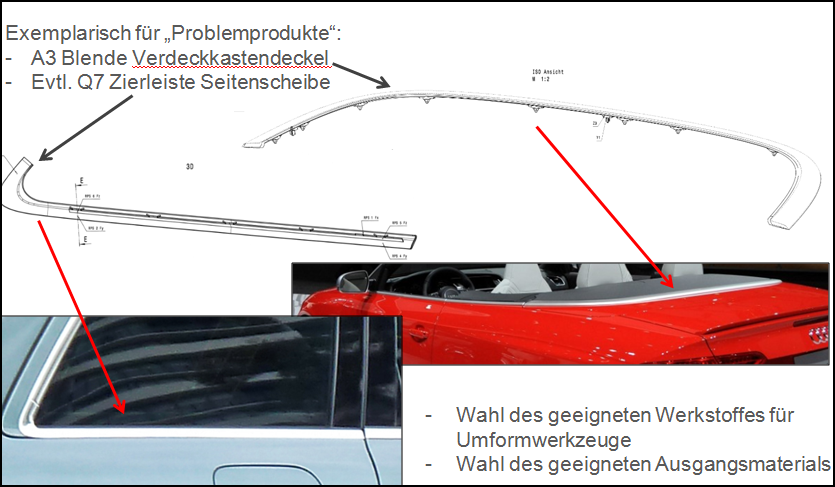
\includegraphics[scale=.7]{ZierleisteVerdeckklappendeckel}
 \caption{Problemprodukte Zierleisten und Verdeckkastendeckel}
 \label{fig:Verdeckkastendeckel}
 \end{figure}

Die nächsten Abschnitte befassen sich mit der Durchführung und Auswertung von Versuchsreihen die mit Hilfe von Messungen, herkömmlicher sowie zukunftsweisender Art (FEM-Verfahren), Erkenntnisse liefern  die die Herstellungsverfahren von Zierleisten  in qualitativer- sowie ökonomischer Sicht  optimieren.\\
Zur Untersuchung   sind hier vor allen Dingen die Umformverfahren  Kröpfen (siehe \fref{sec:kropf})  und Streckbiegen herangezogen worden. 


\newpage

\section{Bauteil}
Prüfobjekt ist in den folgenden Untersuchungen der Verdeckkastendeckel  des Audi A3 Cabriolet's (siehe \fref{fig:audia3}).
 Als Verzierung eines Luxusobjektes sind die Anforderungen an Aussehen und Qualität außergewöhnlich hoch. So dient er zum einen als rein optisches Veredelungselement zum anderen hat er auch funktionelle Aufgaben (z.B. Stabilität in den gesamten Kofferraumdeckel bringen oder auch als Antenne zu agieren). Geringe Spaltmaße,  perfekte Symmetrie (das menschliche Auge erkennt ein Hundertstel Millimeter) so wie allgemeine Benutzerfreundlichkeit (z.B. Hängenbleiben von Kleidungsstücken und ähnlichem and dem Verzierungsobjekt sollte ausgeschlossen sein) sind Anforderungen die höchste Priorität haben.
 Darüber hinaus sind  flüssige Übergänge und Einklang   zu weiteren Verzierungselementen des Fahrzeuges primordial für einen harmonischen Gesamteindruck.
 
   
\begin{figure}[!htb]
\centering
\hfill
\subfloat[Audi A3 ]{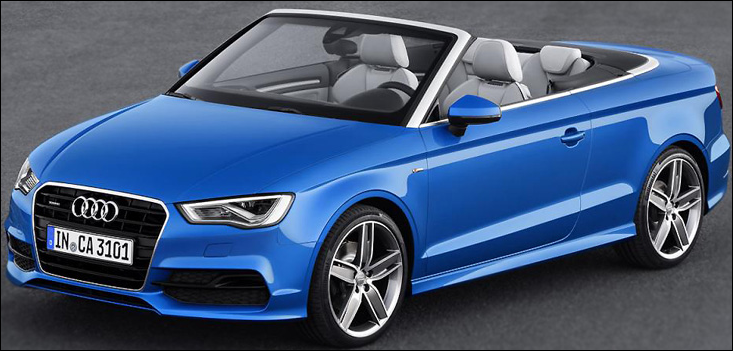
\includegraphics[scale=.4667]{audia3blau}}
\hfill
\subfloat[Audi A3 Verdeckkastendeckel \label{fig:audia3verdeck}]{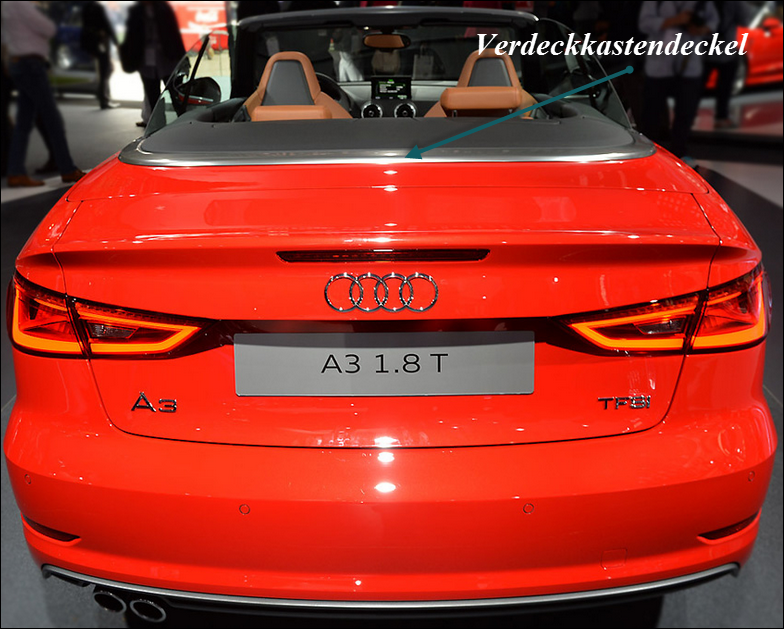
\includegraphics[scale=.263]{audivdkd}}
\hfill
\caption[Audi A3 Endprodukt]{Audi A3 Endprodukt\footnotemark }
\label{fig:audia3}
\end{figure}
 \footnotetext{Vgl.http://www.cars.co.za/motoring\_news/2014-audi-a3-cabriolet-completes-the-a3-family/6061/[28.12.2013].}



	 	 
\subsection{Funktion \& Qualitätsumfang}
An Verzierungselemente werden gerade in der Automobil Oberklasse besonders hohe Ansprüche gestellt. Es sind besonders folgende hervorzuheben:
\begin{itemize}
\item keine Beulen
\item keine Oberflächenfehler
\item ideale Fugenläufe
\item präzise Radien
\item enge Form- und Lagetoleranzen (siehe \fref{fig:vdkdtol})
\item enge Spalttoleranzen
\end{itemize}
\begin{figure}[!htb]
  \centering
  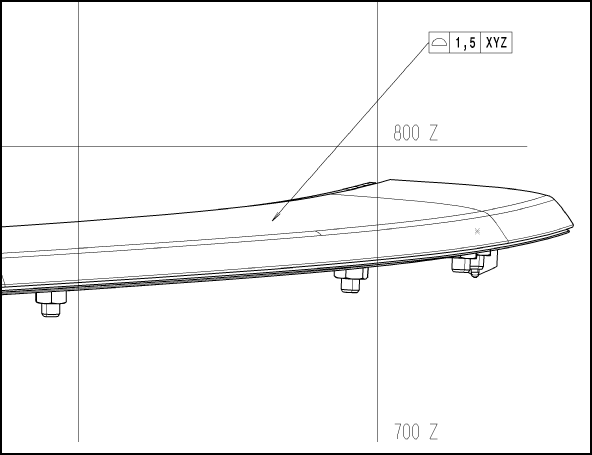
\includegraphics[width=1\linewidth,height=.2\textheight] {vdkdtol}
  \caption{Wölbungstoleranz}
  \label{fig:vdkdtol}
  \end{figure}






\subsection{Aluminium}
Aufgrund seiner geringen Dichte (\SI{2.69}{\kilo\gram\per\deci\meter\cubed})\footcite[Vgl.][353]{wm}, guten Umformbarkeit, Korosionsbeständigkeit und mit einer hervorragend zu erzielender Oberflächengüte sowie hohem Reflexionsgrad ist Aluminium das am häufigsten verwendete Ausgangsmaterial für Zierleisten.\\
 Es werden überwiegend Strangpressprofile verarbeitet die bei den Lieferanten mit bestimmten Eigenschaften angefordert werden. Die wichtigsten dort angeführten mechanischen Eigenschaften sind die Zugfestigkeit $R_m  [\si{\newton\per\milli\meter\squared}$], Dehnung $R_{po,2} [\si{\newton\per\milli\meter\squared}]$,   Bruchdehnung A oder auch $A_{50} [\si{\percent}]$ (der Index 50 bezieht sich auf eine Messlänge  von \SI{50}{\milli\meter} der Probe  beim einachsigen Zugversuch)\footcite[Vgl.][281]{aa}und die Korngröße.\\
  Sie wird in der Einheit [\si{\micro\meter\squared}] angegeben und hat Einfluss auf die Oberflächengüte nach  Umformprozessen. Bei steigendem Umformgrad ergibt sich häufig eine Aufrauung der Oberfläche (Orangenhaut) die von der Ausgangskorngröße abhängig ist. Je geringer die Ausgangskorngröße desto geringer der Aufrauungseffekt.\footcite[Vgl.][524]{aa}\\
Erwähnenswert ist zu vorangegangenem noch das aufgrund der, bei den meisten Aluminiumlegierungen, nicht ausgeprägten Streckgrenze  die $R_{p0,2}$ Dehngrenze als Bemessungskennwert bei einer \SI{0.2}{\percent} bleibenden Verformung gegenüber rein elastischem Verhalten ermittelt wird (siehe \fref{fig:spanndehn2}).\footcite[Vgl.][280-281]{aa}  
\begin{figure}[h!tbp]
\centering
 	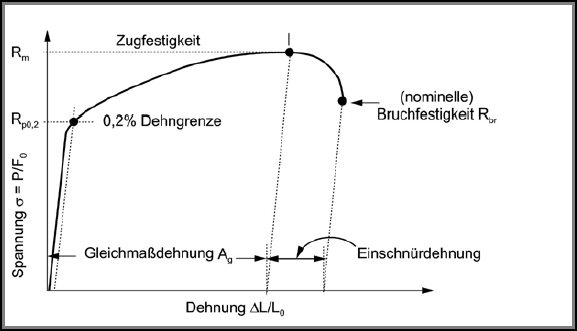
\includegraphics[scale=.9]{spanndehn2}
 	\caption{Spannungs-Dehnungs Schaubild mit $Rp_{0,2} $ Dehngrenze}
 	\label{fig:spanndehn2}
 	\end{figure}
	 	 	 	 
	 	 	 	 

\subsection{Streckbiegen}
Bei dem Umformverfahren Streckbiegen werden auf speziellen Streckbiegemaschinen die Enden eines Profilstranges in Spannern gehalten und auf  Zugspannung gebracht (siehe  \fref{fig:Streckbiegemaschine}). Anschließend werden sie über ein massives Biegewerkzeug streckgebogen.\footnote{Vgl.\url{http://www.tillmann-gruppe.de/de/streckbiegen.html}[27.10.2013].}
\begin{figure}[!htb]
\centering
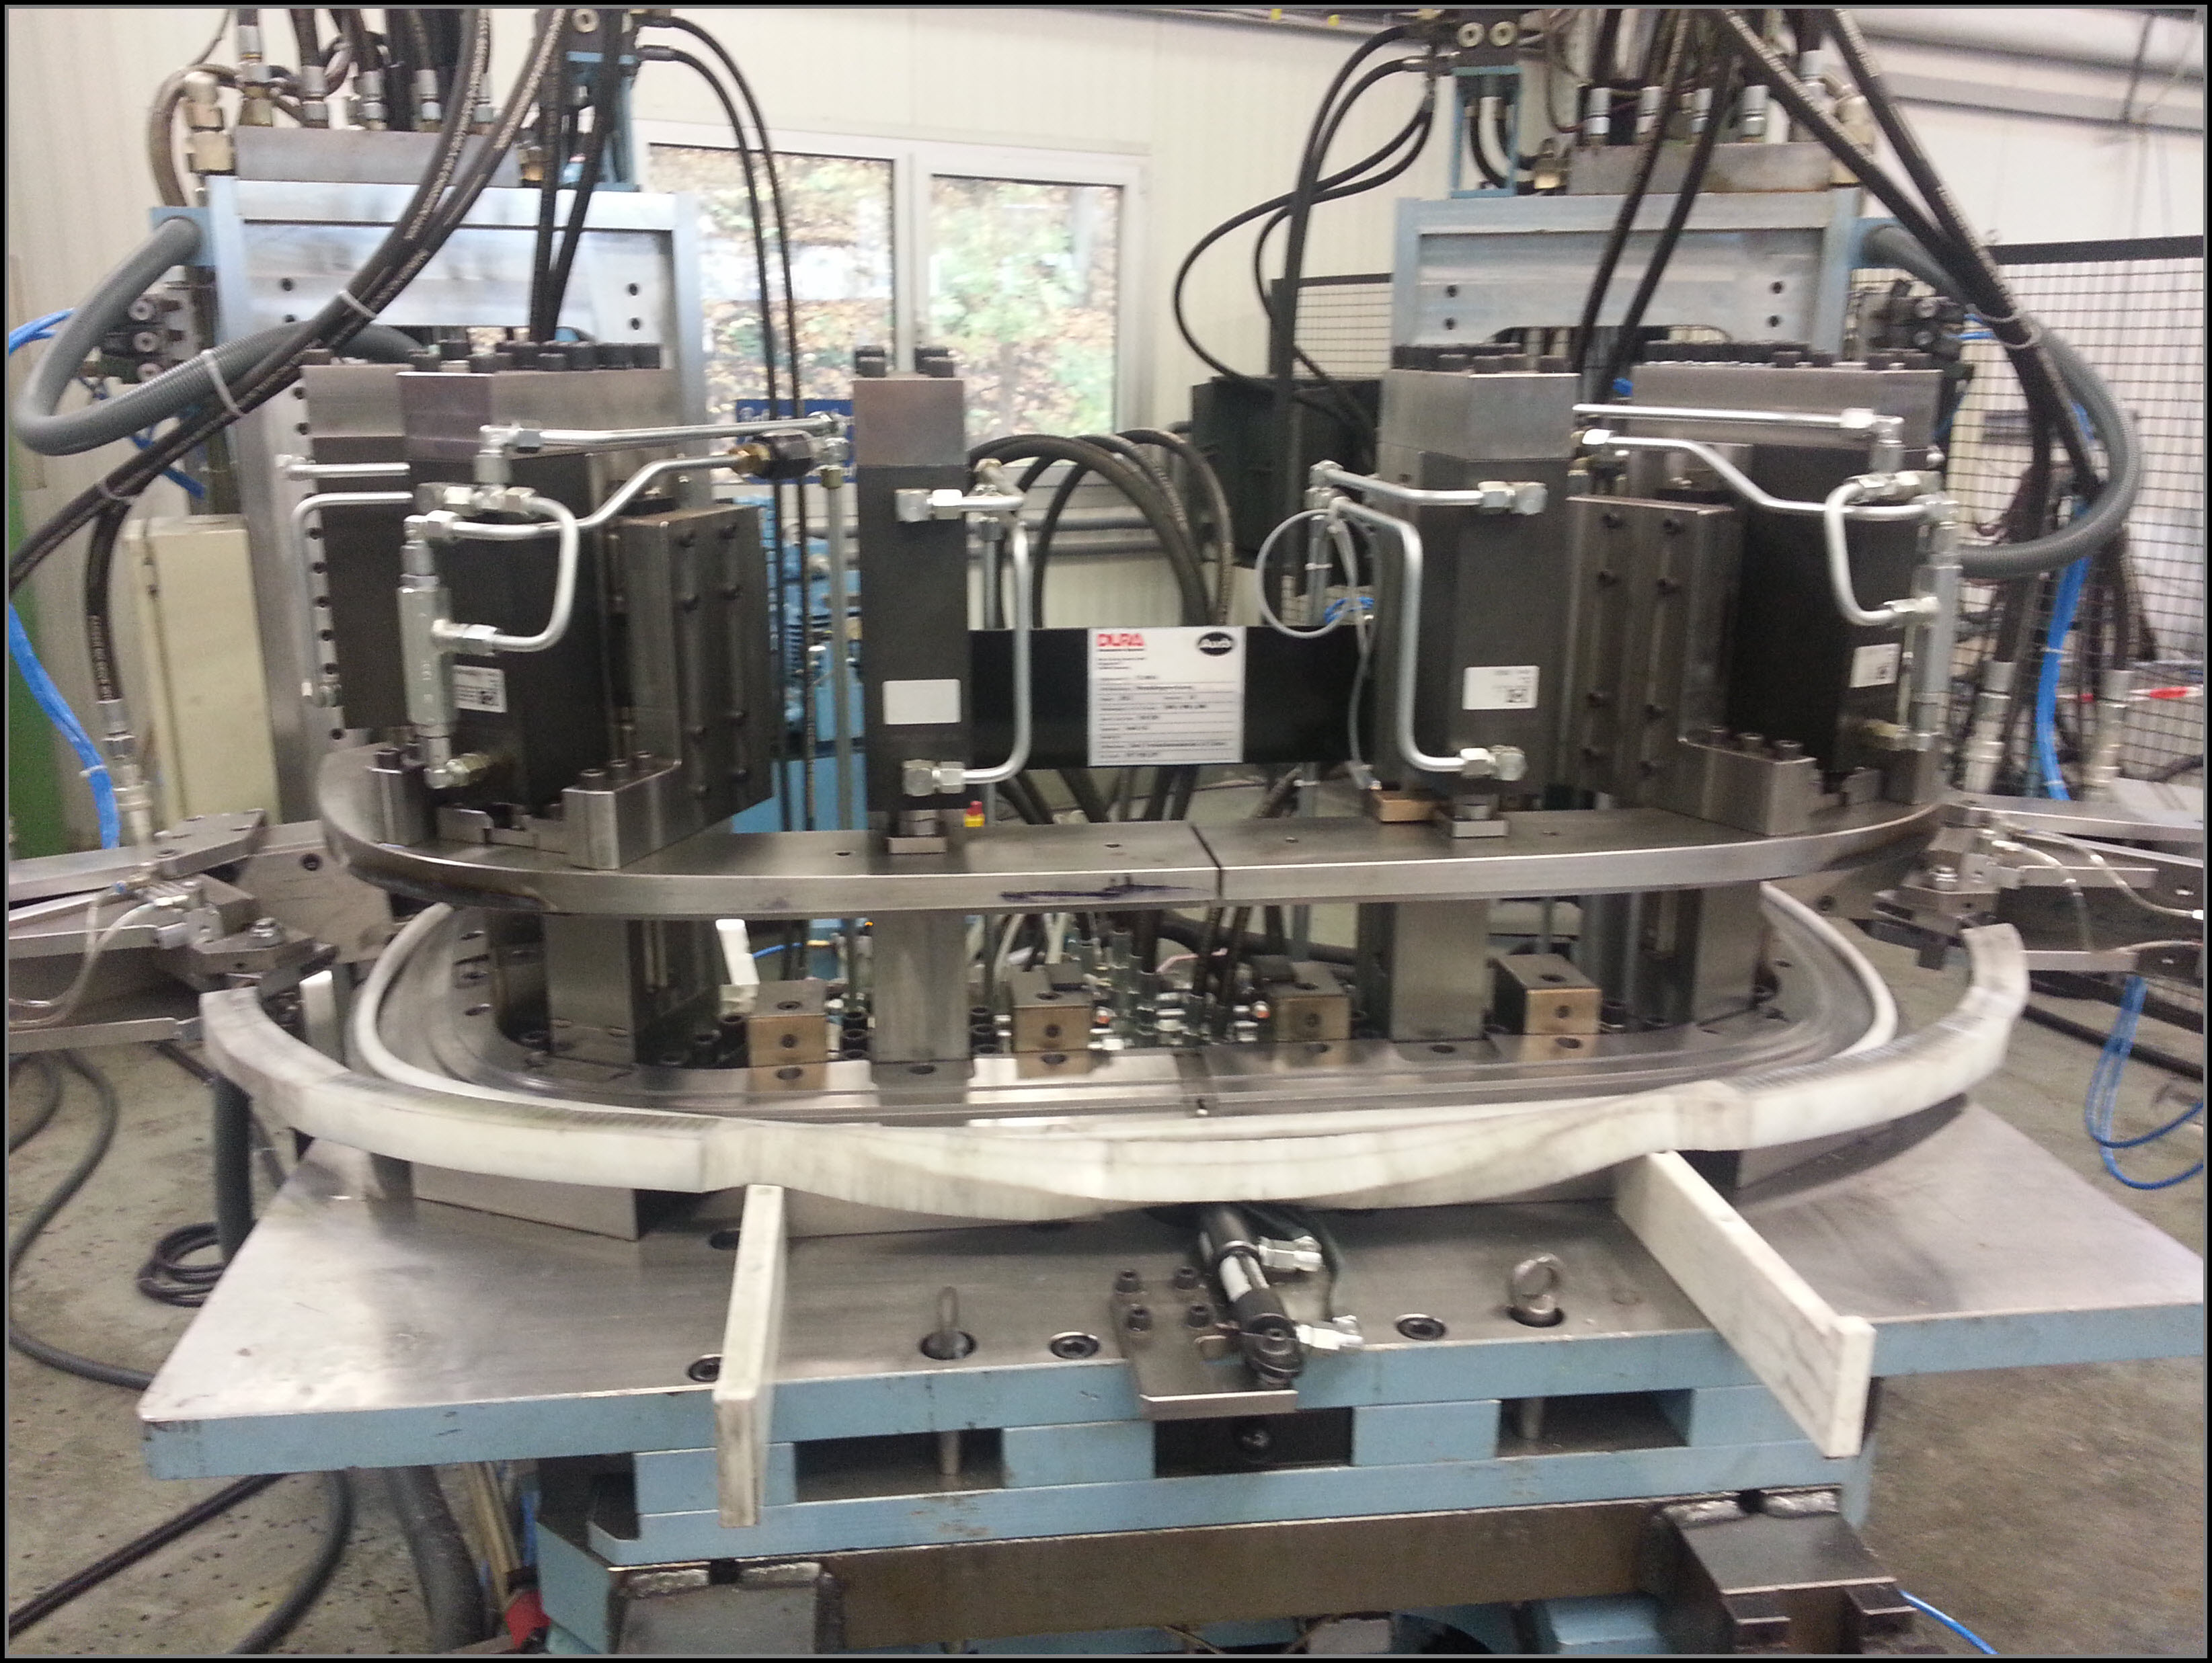
\includegraphics[scale=.12]{Streckbiegemaschine}
\caption{Streckbiegemaschine}
\label{fig:Streckbiegemaschine}
\end{figure}
Das Ausgangsmaterial (Aluminium Strangpressprofile) wird streckgebogen um eine Rückfederung zu minimieren. Kritisch sind hier vor allen Dingen Biegeschwankungen und nicht kontinuierliche Materialeinschnürungen,  welche häufig an den Verengungen der Biegeradien auftreten. Die einflussreichsten mechanischen Eigenschaften des Werkstoffes sind bei diesem Verfahren die Härte sowie die Streckgrenze.

\subsection{Kröpfen \label{sec:kropf}}
Der eigenartig anmutende Ausdruck \emph{Kröpfen} bedeutet eigentlich nur \emph{krumm biegen}\footnote{Vgl.\url{
http://woerterbuchnetz.de/DWB/?sigle=DWB&mode=Gliederung&lemid=GK14769
}[27.10.2013].}
Bei dem Umformprozess Kröpfen werden von den  Enden der Zierleisten zu nächst die auf den Innenseiten verlaufenden Stege  abgefräst.  Daraufhin werden sie in der Kröpfeinheit (siehe \fref{fig:kropfeinheit}) auf dem Kröpfstein justiert und von einem Niederhalter durch die Anpresskraft einer Gasdruckfeder angepresst. Nun fährt, angetrieben durch einen Hydraulikzylinder, der Kröpf- oder auch Ziehstempel herunter und kantet das Material ab. Im Anschluss daran wird die Stirnseite der Kröpfung (siehe \fref{fig:kropfinstirn}) noch beschnitten.
\begin{figure}[!htb]
\centering
\hfill
\subfloat[Bezeichnungen \label{fig:kropfeinhzeich}]{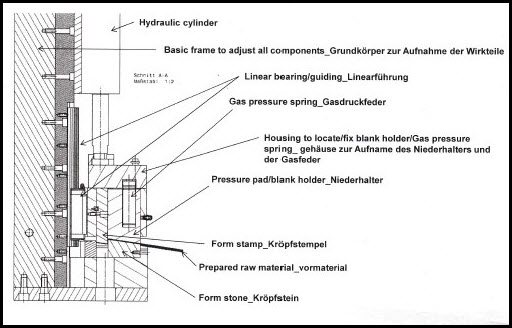
\includegraphics[scale=.68]{kropfeinhzeich}}
\hfill
\subfloat[Kröpfstein\label{fig:einheit}]{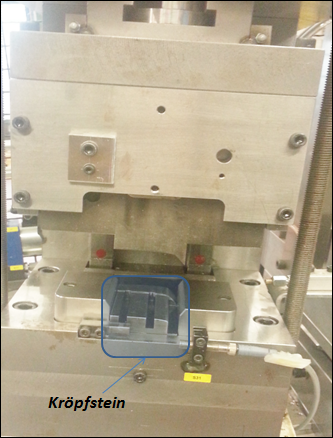
\includegraphics[scale=.5]{kropfeinheit}}
\hfill
\caption{Kröpfeinheit }
\label{fig:kropfeinheit}
\end{figure}

\begin{figure}[!htb]
\centering
\hfill
\subfloat[Kröpfung mit Fräsbereich  \label{fig:kropffrasbereich}]{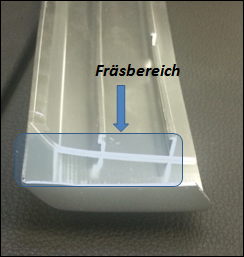
\includegraphics[scale=.822]{kropffrasbereich}}
\hfill
\subfloat[Kröpfung \label{fig:kropfung}]{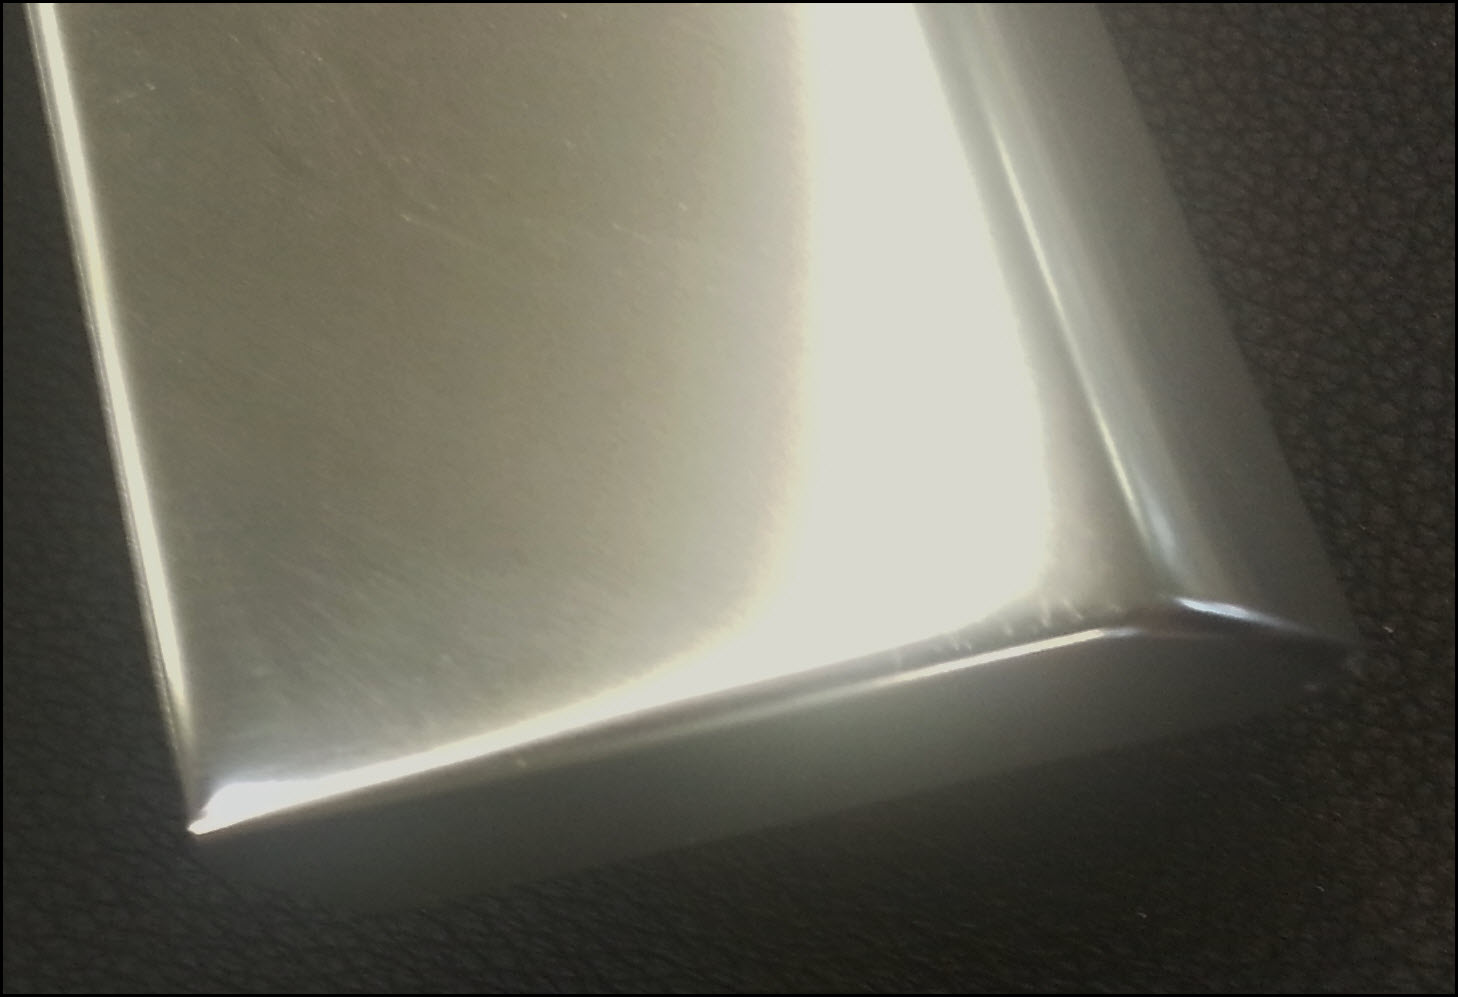
\includegraphics[scale=.16]{kropfung}}
\hfill
\caption{Kröpfung innen und Stirnseite }
\label{fig:kropfinstirn}
\end{figure}


 
Problembereiche sind hier zu erst einmal die Fräsprozesse. Schon bei geringsten Unterschieden in der Materialabnahme sind Fehlstellen in der Oberflächenqualität der Radien bei einer Sichtprüfung zu erkennen. Auch der Ziehstempel und der Kröpfstein lassen Spuren auf der Oberfläche zurück. Ein nicht zu vernachlässigender Aspekt sind auch Verschleiß des Werkzeugmaterials bei diesem Verfahren. So kommt es gerade bei Ziehstempeln aus Stahl oft zu Kaltaufschweißungen. Hier liegt nahe auch andere Werkzeugmaterialien in Versuchsreihen zu erproben.
\medskip

Hervorzuheben sind folgende, aus dem Kröpfprozess resultierende, Qualitätsbeeinträchtigungen:
\begin{itemize}
\item Orangenhaut
\item Materialungänzen bedingt durch Materialschwankungen
\item Abweichungen des auf das Kröpfen angepassten Fräsbildes
\end{itemize}











\subsection{Methode Messauswertung}
Es wurde bei der Auswertung von Messreihen in dieser Untersuchung vorwiegend die \textbf{\emph{empirische}} Standardabweichung $ s= \sqrt{\frac{\sum \limits_{i=1}^n (x_i - \bar{x})^2}{n-1}}$ verwendet, welche für solche Operationen von der Fachliteratur empfohlen wird.\footcite[Vgl.][301]{mf} Der Unterschied zur Standardabweichung $ \sigma = \sqrt{\frac{\sum \limits_{i=1}^n (x_i - \bar{x})^2}{n}}$ ist das \emph{Teilen} durch \textbf{n-1} anstatt durch lediglich \textbf{n}.
 An dieser Stelle eine kurze Beleuchtung des Sachverhaltes  (in Anbetracht der Erläuterungen von Dr. Guido Pinkernell\footnote{\url{www.ti-unterrichtsmaterialien.net/imgserv.php?id=pinkernell_106.pdf}[10.11.2013].‎}, welche exzellent  den Sachverhalt beleuchten)\footnote{Herv. d. Verf.}.



Die \textbf{\emph{empirische}} Standardabweichung berechnet das Streuungsmaß einer \emph{Stichprobe} im Gegensatz zur Standardabweichung die sich auf eine \emph{Grundgesamtheit} bezieht. Bei Stichproben wir die \emph{empirische} Standardabweichung vorgezogen da dort in der Regel die \emph{wirkliche Streuung} unterschätzt wird. Die \emph{empirische} Standardabweichung ist wegen des Teilers n-1 grundsätzlich etwas größer als die Standardabweichung, bei großem n liefern aber beide nahezu gleiche Ergebnisse, welches ja nur eine logische Konsequenz ist, denn je größer die Stichprobe desto näher kommt sie an die Grundgesamtheit.

\medskip

Durch das Quadrieren der einzelnen Abweichungen ($ x_i-\bar{x}$) und Addieren der einzelnen Abweichungsquadrate erhält man nur positive Beträge in denen eine Überbetonung einzelner Ausreißer erzielt wird.
Die empirische Standardabweichung ist   eines der wichtigsten Vergleichsparameter in der Statistik und bietet sich zur Analyse der Versuchsreihen besonders an, da sie von Extremwerten nicht stark beeinflusst wird.\footcite[Vgl.][54]{gst} Bei der Auswertung von Messbereichen, die für unsere Problemstellung besondere Signifikanz haben, wird zusätzlich der Fehler mit Hilfe der  \emph{Standardabweichung des Mittelwertes}  $ \Delta\bar{x}= t_{0,95} \cdot \sqrt{\frac{\sum \limits_{i=1}^n (x_i - \bar{x})^2}{(n-1)\cdot n}}$ angegeben.\footcite[Vgl.][16]{ph} Da bei den Versuchsserien eine nicht allzu große Stückzahl ($ n=16-20 $) bearbeitet wurde,  ist auch der für die international geforderte statistische Sicherheit zu berücksichtigende \emph{P} Wert mit dem $ t_{0,95} $ Faktor in die Berechnungen eingegangen.\footcite[Vgl.][609]{tp}  Es sei noch bemerkt, dass der Fehler nach DIN 1333 jeweils auf die erste signifikante Stelle gerundet wurde.\footcite[Vgl.][612]{tp}
 	 	
 	

 	
 	 	


\subsection{Chargenvergleich Streckbiegen}
Zur Versuchsdurchführung wurden drei Materialchargen zu jeweils 20 Profilen des Werkstoffes EN AW 6060 (Legierungsnummer EAL-6048 \emph{Alminox}, AlMgSi\,0,5) mit den Materialbezeichnungen F17 (T61/Charge 1) und Fxx (T4/Charge 2) sowie das ursprünglich zur Serienfertigung vorgesehene Material F13 (T4)  gegenübergestellt (eine Übersicht der relevantesten Eigenschaften ist in \fref{tab:chargeneigenschaften} aufgeführt).
\begin{table}[htbp]
\caption{Gegenüberstellung der mechanischen Eigenschaften (Laborwerte) der Chargen}
\label{tab:chargeneigenschaften}
\centering
\begin{tabular}{lllll}
\toprule
Material & Zugfestigkeit & Streckgrenze & Bruchdehnung & Zustand \\
Charge &  Rm [\si{\newton\per\milli\meter\squared}] &  $R_{p0,2}$ [\si{\newton\per\milli\meter\squared}] &  $A_{50}$ [\%] & \\
\midrule
1.F17 & 160,25 & 85,55 & $ 12,3 $ & T61 \\
2.Fxx & 152,4 & 74,65 &  $ 11,65 $ & T61 \\
3.F13 Serie & 149,3 & 70,55 & 20,41  & T4 \\
\bottomrule




\end{tabular}
\end{table}


 Die Chargen 1 und 2 wurden auch mit der herkömmlichen Zustandsbezeichnung T61 (lösungsgeglüht, nicht vollständig warmausgelagert, überaltert)\footnote{Vgl.\url{http://www.unibw.de/lrt5/lehre/praktikum/zusatzinformationen/download4/at_download/down1}[25.11.2013].} bezeichnet während das Serienmaterial im Zustand T4 (lösungsgeglüht, kaltausgelagert) bestellt wurde. \\
 Unter Überalterung versteht man  den Prozess der Vereinigung von  submikroskopischen Ausscheidungen die sich  in der Anzahl verringern jedoch als Ausscheidung größer werden und so eine Abnahme der Festigkeit herbeiführen.\footcite[Vgl.][52]{wki}\\
  Lösungsglühen erfolgt durch Glühen im Bereich der homogenen Mischkristalle welches das   Lösungsvermögen der Mischkristalle begünstigt, Ausscheidungen können so gelöst werden.\\
   Unter Auslagern versteht man Liegenlassen bei Raumtemperatur (Kaltauslagern) oder bei  höheren Temperaturen (Warmauslagern), meistens zwischen 100 und 220 Grad Celsius, über einen bestimmten Zeitraum um so die Eigenschaften des Werkstoffes zu beeinflussen.\footcite[Vgl.][213]{wk}
Ein typischer Aushärtungsprozess läuft nach folgendem Schema ab:

\begin{enumerate}
 \item Lösungsglühen aller Ausscheidungen in einem homogenen Mischkristall 
 \item Abschrecken
 \item Auslagern 
 \end{enumerate}
 
   
 
 

Die Zusstandsbezeichnungen F17, F13 und Fxx beziehen sich nach DIN 755-2 auf die Zugfestigkeit. Fxx ist allerdings eine firmeninterne Bezeichnung und bedeutet das ein  vorgezogener Kaltauslagerungsprozess durchgeführt wurde um das Strangpressprofil zu "`\emph{stabilisieren}"'. Das bedeutet ein gewisses "`Einfrieren"' des Gefüges in den momentanen Zustand um Veränderungen desselbigens auch bei nicht vorgesehener längerer Lagerung zu verhindern. Nach Auskunft des Lieferanten ist Fxx leicht wärmebehandelt worden.


 Bei Charge 2 (Fxx) schieden zwei Profile aufgrund von Biegefehlern aus. Die Proben wurden streckgebogen und auf einer Messlehre  mit 40 Messpunkten (Messpunkte MP1a bis MP10d) vermessen. Die Messbereiche, Messpunkte und Messuhren wurden, zur besseren Übersicht, mit Farben markiert (siehe \fref{fig:messpunktevdkda3}).  \\
 And den Messpunkten wurden folgende Messbereiche ermittelt:
 \begin{description}
 \item[MP1a-MP10a] Kontur aussen (grün)
 \item[MP1b-MP10b] Spalt (gelb)
 \item[MP1c-MP10c] Wölbung oben innen (rot)
 \item[MP1d-MP10d] Wölbung oben aussen (blau)
 \end{description}
\begin{figure}[!htb]
\centering
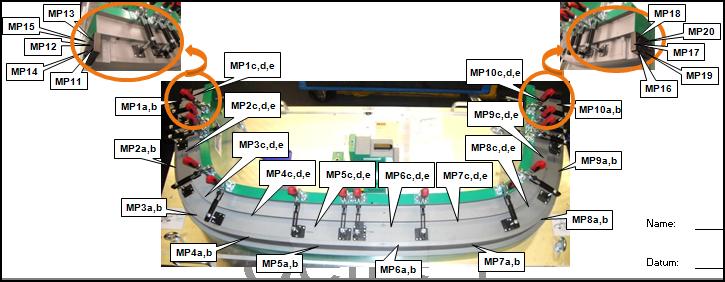
\includegraphics[width=1\linewidth,height=.2\textheight]{messpunktevdkda3}
\caption{Messpunkte Biegelehre}
\label{fig:messpunktevdkda3}
\end{figure} 
 
 
 
 
Das Messen erfolgte durch Abfahren aller Messpunkte mit den zu den spezifischen Messbereichen zu verwendenden Messuhren (siehe \fref{fig:messverfahren}). Ein negativer Messwert lässt auf eine Verkleinerung des Messbereiches schließen. Eine Ausnahme hierzu ist der Messbereich "`\emph{Spalt vorne unten}"' welcher  bei negativen Werten eine Vergrößerung bedeutet.\\
 Alle relevanten Messergebnisse (mit Ausnahme der Messpunkte MP1b und MP10b bei Charge 1, welche nicht zu ermitteln waren) wurden in Tabellen eingetragen und  der Mittelwert sowie die Standardabweichung
 ermittelt. Darüber hinaus erfolgte eine Gegenüberstellung der spezifischen Werte.\\
Da aufgrund der vielen Messpunkte  sehr umfangreiche Auswertungen durchgeführt wurden,  sind hier die für die Problematik Ausschlaggebendsten näher betrachtet worden. Alle weiteren Messergebnisse und Visualisierungen sowie Dokumentationen sind dem Anhang zugefügt. 
\begin{figure}[!htb]
\centering
\hfill
\subfloat[Messlehre  \label{fig:messlehre}]{\includegraphics[scale=.0877]{Messlehre}}
\hfill
\subfloat[Messung "`Kontur aussen"' \label{fig:messvdkd}]{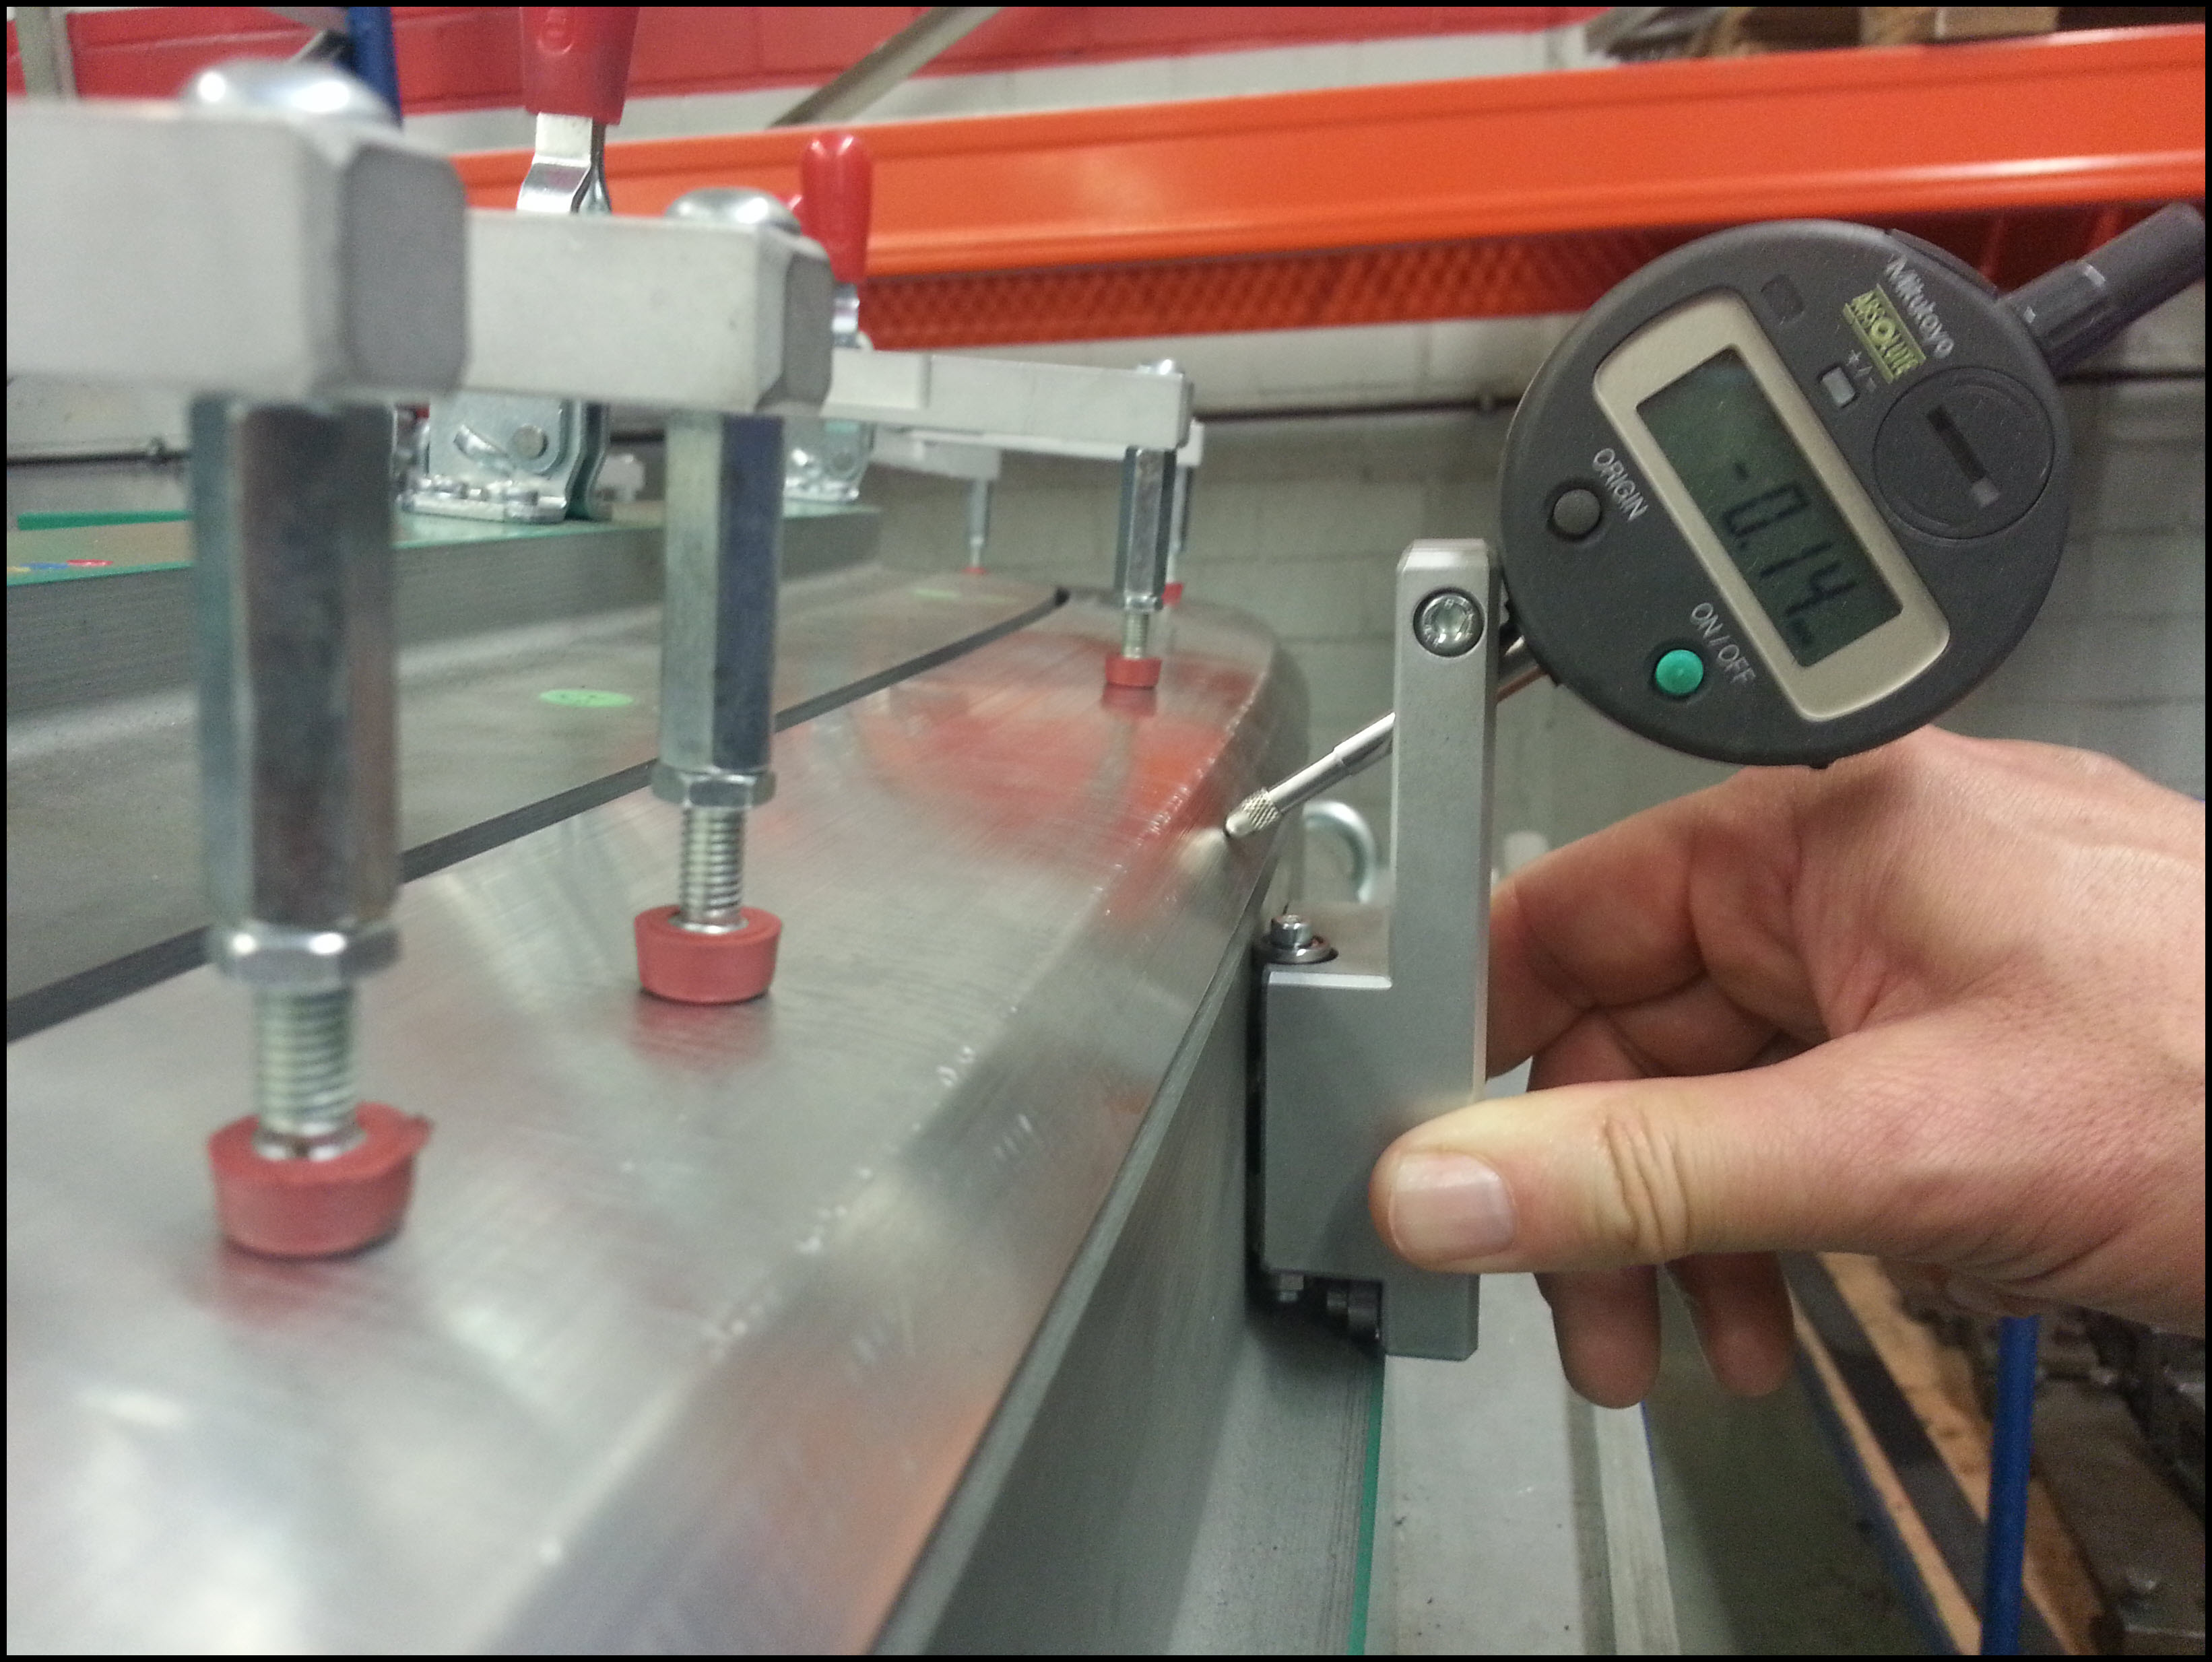
\includegraphics[scale=.042]{messvdkd}}
\hfill
\caption{Messverfahren an der "`Biegelehre"' }
\label{fig:messverfahren}
\end{figure}


Der für das Streckbiegen aussagekräftigste Parameter ist der Messbereich "`\emph{Kontur aussen}"' da er dem Verlauf der Biegelinie entspricht. Besonders an den Messpunkten MP1a und MP10a sind die Auswirkungen der Rückfederung zu beobachten. Ein Vergleich der Chargen ist in \fref{tab:mwertstandstreck} übersichtlich dargestellt. Ein visueller Vergleich der Standardabweichungen der "`Kontur aussen"' ist in \fref{fig:svstb} aufgeführt.
\begin{figure}[!htb]
\centering
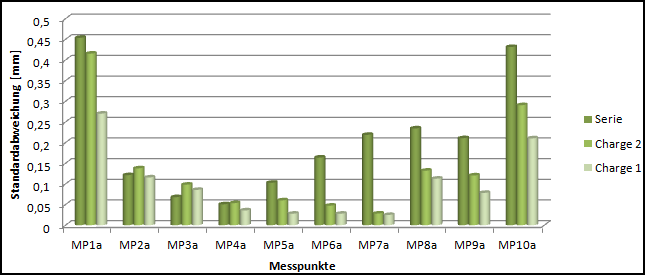
\includegraphics[width=1\linewidth,height=.3\textheight]{standardstreckb}
\caption{Überlagerung Standardabweichungen "`Kontur aussen"' Streckbiegen}
\label{fig:svstb}
\end{figure}
Dort ist zu sehen, dass das Material F17 (Charge 1) an fast allen Messpunkten die geringste Standardabweichung aufweist. Lediglich bei Messpunkt MP3a liegt sie in nicht großem Abstand zwischen dem Fxx (Charge 2) und dem F13 (Serie) Material.

Ein Vergleich der Mittelwerte (Kontur aussen) der Chargen (siehe  \fref{fig:mitstrckb}) ergibt, dass and den Messpunkten MP1a, MP2a, MP9a und MP10a  Charge 1 (F17) die größte Rückfederung nach dem Streckbiegeprozess auftritt.






\begin{table}[htbp]
\caption{Messwerte und Standardabweichungen Streckbiegen "`Kontur aussen"'} 
\label{tab:mwertstandstreck}
\vskip\abovecaptionskip



\footnotesize
   \begin{tabular}{cccccc}
   \toprule
   & \multicolumn{5}{c}{Messwert $x =  (\bar{x} \pm \Delta x)  $[mm]}\\
   \cmidrule(ll){2-6}
   Material    & MP1a & MP2a & MP3a & MP4a & MP5a \\  
   
   \midrule
  
   F17& $ 1,95\pm 0,13 $ & $0,72 \pm 0,06 $ & $0,60 \pm 0,04 $ & $ 0,028 \pm 0,017 $ & $-0,297 \pm 0,014$ \\
    Fxx & $0,81 \pm 0,21 $ & $0,34 \pm 0,07 $ & $0,15 \pm 0,05 $ & $0,021 \pm0,027 $ & $ -0,188\pm0,030$ \\
   F13  Serie & $-0,66 \pm0,22 $ & $-0,13 \pm 0,06 $ & $-0,38 \pm 0,04$ & $ 0,028\pm0,024 $&$0,00 \pm0,05 $ \\
     \bottomrule
     \toprule
  Material   & MP6a & MP7a & MP8a & MP9a & MP10a  \\
  \midrule
      F17&   $-0,368 \pm0,014 $&$-0,293 \pm0,012 $&$ 0,46 \pm 0,06 $&$ 1,31\pm 0,04$&$2,96 \pm0,10 $ \\
Fxx &$-0,233 \pm0,024 $&$-0,251 \pm0,015 $&$-0,17 \pm0,07 $&$0,57 \pm0,06 $&$1,37 \pm0,15 $ \\
  F13 Serie & $-0,04 \pm0,08 $&$ -0,16\pm0,11 $&$-0,55 \pm0,11 $&$0,04 \pm  0,10$&$-0,08 \pm0,21$ \\
     
     \bottomrule
      
     &&&&&\\
     &&&&&\\
     &&&&&\\
     &&&&&\\
     &&&&&\\
     
     \toprule
      & \multicolumn{5}{c}{Standardabweichung s [mm]}\\
   \cmidrule(ll){2-6}
   Material    & MP1a & MP2a & MP3a & MP4a & MP5a \\ 
   \midrule
    F17&0,270&0,116&0,086&0,036&0,028\\
    Fxx &0,416&0,138&0,098&0,053&0,060\\
    F13 Serie&0,454&0,121&0,068&0,051&0,103\\
     \bottomrule
     \toprule
  Material    & MP6a & MP7a & MP8a & MP9a & MP10a  \\
  \midrule
    F17 &0,028&0,025&0,113&0,078&0,210\\
 Fxx   &0,048&0,028&0,132&0,121&0,291\\
F13 Serie &0,164&0,219&0,235&0,211&0,432\\ 
   \bottomrule 
         
   \end{tabular} 
\end{table}

\begin{figure}[!htb] 
\centering
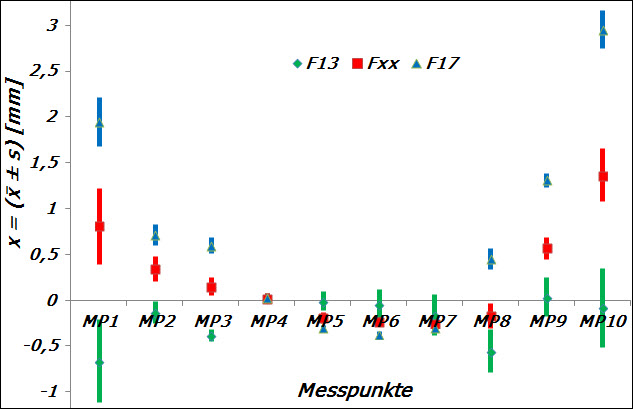
\includegraphics[width=1\linewidth,height=.3\textheight]{mitkontausstrckb}
\caption{Vergleich Mittelwerte "`Kontur aussen"' Streckbiegen}
\label{fig:mitstrckb}
\end{figure}

\newpage

\subsubsection{Ausblick}
In folge der Überlagerung der Standardabweichungen (Streckbiegen "`Kontur aussen"') der untersuchten Chargen unter dem Gesichtspunkt der Mindestzugfestigkeiten (siehe \fref{fig:standzugrel}) ist einzusehen, dass das Material F17 (Charge 1) bei einer Mindestzugfestigkeit von Rm = 160  \si{\newton\per\milli\meter\squared}  die geringste Standardabweichung hat. Bei Werten von s = (0,025  bis 0,270) \si{\milli\meter}  ist davon auszugehen das auch größere Stückzahlen mit relativ geringen Prozessschwankungen zu fertigen sind. Hier müssen jedoch eventuelle Montageprobleme des Verdeckkastendeckels aufgrund der höheren Rückfederungswerte von {$x_{\text{Rückfeder}}$ = (-0,368  bis 2,96) \si{\milli\meter} berücksichtigt werden. Eine Tatsache die bei einer Spannweite von 3,328 \si{\milli\meter} schon einen beachtlichen Spielraum beim Einbau und bei der Passform bedarf.  % montage wegen der Toleranzen fragen
Hier ist das Ausmaß von Wölbungen und Spannungen nach und während der Montage schon genau zu untersuchen.

\begin{figure}[!h]
\centering
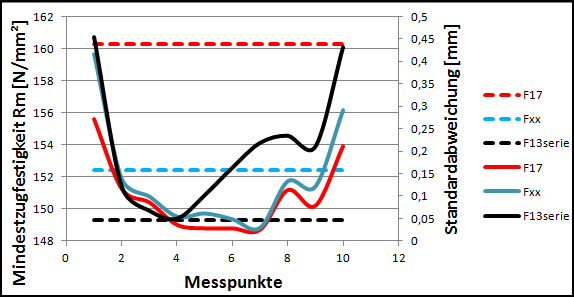
\includegraphics[width=1\linewidth,height=.3\textheight]{standzugrel}
\caption{Übersicht Mindestzugfestigkeit/Standardabweichung "`Kontur aussen"'}
\label{fig:standzugrel}
\end{figure} 

Zu einem ähnlichen Ergebnis kommen wir bei Betrachtung der Überlagerung der Chargen unter Berücksichtigung der Standardabweichung im Bezug zur Streckgrenze (siehe \fref{fig:standstreckrel}).
\begin{figure}[!h]
\centering
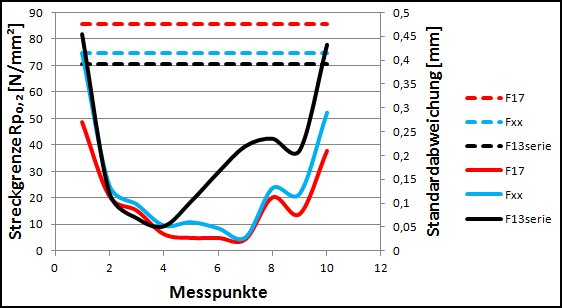
\includegraphics[width=1\linewidth,height=.3\textheight]{standstreckrel}
\caption{Übersicht Streckgrenze/Standardabweichung "`Kontur aussen"'}
\label{fig:standstreckrel}
\end{figure} 
Unter der Voraussetzung geringer Prozessschwankungen im Streckbiegeverfahren welche bei geringer Standardabweichung unter sorgfältiger und präziser Auswahl des Vormaterials durchaus zu realisieren sind, können die Ausschussrate sowie Kosten und Zeitverluste die durch ständiges Justieren der Streckbiegemaschine durch geschultes Personal entstehen, erheblich reduziert werden.

In Anbetracht der vorangegangenen Auswertung wurden noch einmal zwei Chargen (F19 und F18) bei dem Zulieferer, zu Versuchszwecken, bestellt. Möglicherweise ist hier ein Material herauszukristallisieren welches noch geringere Prozessschwankungen ermöglicht. Wir sind dabei von einer steigenden Zugfestigkeit ausgegangen da sich nach den Diagrammen in \fref{fig:standzugrel} und \fref{fig:standstreckrel} die Standardabweichung sowie Mindestzugfestigkeit und Streckgrenze gegenläufig verhalten.

\section{Exkurs Umformtechnik}


Da die Gegenstände und Verfahren dieser Untersuchung in das Gebiet der Umformtechnik fallen werden die ausschlaggebendsten Begriffe und Sachverhalte dieses komplexen Gebietes noch einmal genauer umrissen. So ist es möglich über ein theoretisches Gerüst zu verfügen welches später behilflich sein wird   Analogien zu den durchzuführenden Prozessen zu erkennen.
\subsection{Systematisierung Formgebungsverfahren}
Umformverfahren können
auf Grund der unterschiedlichen Spannungsverhältnisse in fünf verschiedene Gruppen unterteilt werden. Einfache Beschreibungen der Spannungsverhältnisse sind kaum möglich denn,  abhängig von der Art der Operation, können  unterschiedliche Spannungen geichzeitig auftreten oder sich sogar  während des Formgebungsvorgangs verändern. Deshalb werden die überwiegenden Spannungen als Klassifikationskriterium ausgewählt. Folgende fünf Gruppen der Umformprozesse werden definiert:
\begin{enumerate}
\item \emph{Druckumformen} nach DIN 8583 behandelt die Formgebung eines festen Körpers  welche den  plastifizierten  Zustand hauptsächlich durch uni- oder multiaxiale Druckbeslastung herbeiführt.
\item \emph{Zugdruckumformen} nach DIN 8584 behandelt die Formgebung eines festen Körpers  welche den plastifizierten Zustand  hauptsächlich durch kombinierte uni- oder multiaxiale Zug- und Druckbelastung herbeiführt.
\item \emph{Zugumformen} nach DIN 8585 behandelt die Formgebung eines festen Körpers welche den plastifizierten Zustand überwiegend durch uni- oder multiaxiale Zugbelastungen verursacht.
\item \emph{Biegeumformen} nach DIN 8586 behandelt die Formgebung eines festen Körpers welche den plastifizierten Zustand hauptsächlich durch eine Biegebelastung herbeiführt.
\item \emph{Schubumformen} nach DIN 8587 behandelt die Formgebung eines festen Körpers welche den plastifizierten Zustand überwiegend durch eine Schubbelastung herbeiführt.

\end{enumerate}

Von untergeordneter Bedeutung sind innerhalb dieser Gruppen  weitere Unterteilungen auf der Grundlagen von kinematischen Überlegungen (z.B. Relativbewegung zwischen Werkzeug und Werkstück), Werkzeug- und Werkstück Geometrien sowie Beziehungen zwischen den beiden möglich. Die Klassifizierung formgebender Methoden unterlässt bewusst die Frage ob ein Prozess durch Erwärmung, bei Raumtemperatur oder weiterer Wärmebehandlung stattfindet. Früher  wurde zur Abgrenzung zwischen Kalt- und Warmformen die Rekristallisationstemperatur gewählt. Obwohl dieses sicherlich das Verhalten  von Werkstückmaterialien während der Formgebung beeinflusst, zählt heutzutage zur Allgemeinerkenntnis das die spontane Erhohlung  eine weitaus größere Rolle in schnellen Umformprozessen spielt. Außerdem führt die herkömmliche Terminologie angesichts der großen Vielfalt  an Materialien die verwendet werden leicht zu Missverständnissen. So würde zum Beispiel die Formgebung von Blei bei Raumtemperatur als \emph{Warmumformen} deklariert während Molybdän bei einer Temperatur von 800 Grad Celsius noch als \emph{Kaltumformen} eingestuft wäre. Aus diesem Grunde unterscheidet DIN 8582 zwischen Formgebung bei Raumtemperatur und Formgebung bei einem auf über Raumtemperatur erwärmten Werkstücks. Überdies ist zu Berücksichtigen ob ein permanenter Temperaturwechsel während des Umformvorgangs stattfindet. Mit Hilfe dieser beiden Kriterien ist eine weiter Unterteilung von den Metall Umformverfahren möglich:

\begin{enumerate}
\item Formgebung nach Erwärmung (Warmumformen)
\item Formgebung ohne Erwärmung (Kaltumformen)
\end{enumerate}

Beide Punkte können weiter eingestuft werden in:

\begin{itemize}
\item Formgebung ohne Veränderung der mechanischen Eigenschaften
\item Formgebung mit temporärer Veränderung der mechanischen Eigenschaften
\item Formgebung mit permanenter Veränderung der mechanischen Eigenschaften
\end{itemize}

In der Industriepraxis kommen letztendlich unzählige Kombinationen der oben aufgeführten Unterteilungen vor.\footcite[Vgl.][2.1ff]{kl}

\subsection{Eigenspannungen}
Das Thema Eigenspannungen im Zusammenhang mit der Verarbeitung von Blechen an die hohe Qualitätsanforderungen gestellt werden ist natürlich von besonderem Interesse bei der Analyse von Problemstellungen die auf den einzelnen Fertigungsstufen entstehen können. Es handelt sich dabei um Spannungen in einem sich im Temperaturgleichgewicht befindenden Bauteil, auf das keine mechanischen Beanspruchungen wirken. Die mit den Eigenspannungen involvierten  Beanspruchungen stehen im mechanischen Gleichgewicht zueinander. Bei Bauteilen und Werkstücken die unter Eigenspannung stehen kann ein Materialversagen wesentlich schneller eintreten da sich die tatsächlich wirkende Spannung aus Eigenspannungen und Spannungen von außen einwirkenden Kräften zusammensetzt. Durch die Eigenspannungen kann auf Grund des daraus resultierenden gestörten Gleichgewichtszustands plastische Formänderung in Form von Verzug auftreten.
Dabei wirken sich Druckeigenspannungen in der Bauteilrandzone meist vorteilhaft aus das sie einer möglichen Rissbildung und Rissausbreitung entgegenwirken.

Es wird im Hinblick auf Auswirkungen auf das Bauteilvolumen eine Unterteilung der Eigenspannungen in drei Gruppen unternommen:
\begin{enumerate}
\item \emph{Makroskopische Eigenspannungen}, welche sich homogen über mehrere Kristallite erstrecken. Bei Störung des Gleichgewichts führen sie zu makroskopischen Formänderungen.
\item \emph{Eigenspannungen}, die in kleinen Abschnitten homogen sind und bei Störungen des Gleichgewichts zu makroskopischen Formänderungen führen.
\item Mikroskopische \emph{Eigenspannungen}, welche durch inhomogene Versetzungsreihen ausgelöst werden und über wenige Atombereiche variieren. Sie tragen nicht zu makroskopischen Formänderungen bei. 


\end{enumerate}

Eigenspannungen werden verursacht durch inhomogene Deformationen im Bauteil, was zu einer weiteren Einteilung führt.

Entstehungsursachen sind:
\begin{itemize}
\item \emph{Thermische Eigenspannungen} (siehe \fref{fig:eigenspanabk})\footcite{hu} die bei Abkühlung eines Bauteils entstehen.\begin{figure}[!htb]
  \centering
  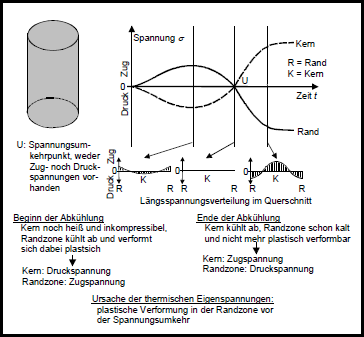
\includegraphics[scale=1.5] {eigenspanabk}
  \caption{Zeitliche Änderung der Längsspannungverteilung im Querschnitt eines Zylinders bei schneller Abkühlung.\footcite[Vgl.][34]{hu}}
  \label{fig:eigenspanabk}
  \end{figure}

\item \emph{Verformungseigenspannungen} (siehe \fref{fig:eigenspanfaser} und \fref{fig:eigenspandrahtzieh}) welche durch inhomogene Verformung auf Grund äußerer Beanspruchung verursacht werden.\begin{figure}[!htb]
  \centering
  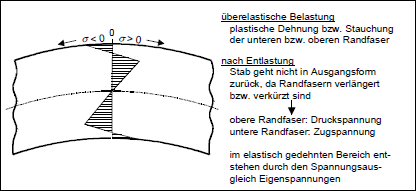
\includegraphics[scale=1.3]{eigenspanfaser}
  \caption{Schematische Längseigenspannungsverteilung im Querschnitt eines Stabs nach plastischer Biegebeansprucheung.\footcite{hu}}
  \label{fig:eigenspanfaser}
  \end{figure}
  \begin{figure}[!htb]
  \centering
  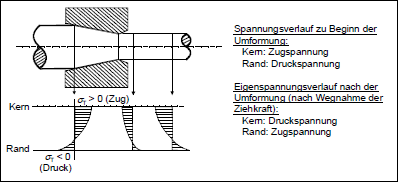
\includegraphics[scale=1.35] {eigenspandrahtzieh}
  \caption{Schematische Tangentialeigensspannungsverteilung beim Drahtziehen in Abhängigkeit von der Ziehdüsenentfernung.\footcite{hu}}
  \label{fig:eigenspandrahtzieh}
  \end{figure}
\item \emph{Umwandlungseigenspannungen} (siehe \fref{fig:eigenspanmol}) die durch inhomogene Gefügeumwandlungen  
mit einer einhergehenden Volumenänderung ausgelöst werden.\begin{figure}[!htb]
  \centering
  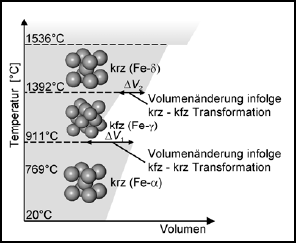
\includegraphics[scale=1.8] {eigenspanmol}
  \caption{Volumenänderung durch Veränderung der Gitterstrucktur. \footcite{hu}}
  \label{fig:eigenspanmol}
  \end{figure}
\end{itemize}











  




 











\newpage
\section*{Anhang}


\printbibliography

\end{document}  